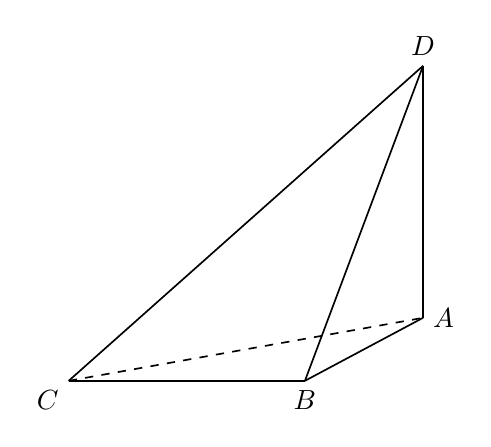
\begin{tikzpicture}[x=1cm,y=1cm,line width=0.6pt,font=\normalsize]
\coordinate (C) at (-3,0);
\coordinate (B) at (0,0);
\coordinate (A) at (1.5,0.8);
\coordinate (D) at (1.5,4);
% solid edges
\draw (C) -- (B);
\draw (B) -- (A);
\draw (B) -- (D);
\draw (D) -- (A);
\draw (D) -- (C);
% hidden edge
\draw[dashed] (C) -- (A);
% labels
\node[below left] at (C) {$C$};
\node[below] at (B) {$B$};
\node[right] at (A) {$A$};
\node[above] at (D) {$D$};
\end{tikzpicture}
